\documentclass[10pt]{article}
\usepackage[utf8]{inputenc}
\usepackage[T1]{fontenc}
\usepackage{amsmath}
\usepackage{amsfonts}
\usepackage{amssymb}
\usepackage[version=4]{mhchem}
\usepackage{stmaryrd}
\usepackage{hyperref}
\usepackage{graphicx}
\usepackage{enumitem}
\usepackage{multirow}
\usepackage{amsthm}
\graphicspath{ {./CS-234/} }

\title{Assignment 4 - Regexes}

\author{CS 234}
\date{Daniel Lee}


\begin{document}
\maketitle

\section*{1 \quad Regexes on Paper}

\begin{enumerate}[label={}]
      \item List the strings of length at most 4 for each of the following languages in shortlex order.


            5.2 $0(0+1)^* 0$

            00, 000, 010, 0000, 0010, 0100, 0110\\

            5.3 $(0+1)^* 0(0+1)^* 1(0+1)^*$

            01, 001, 010, 011, 101, 0001, 0010, 0011, 0100, 0101, 0110, 0111, 1001, 1010, 1011, 1101\\

            5.5 $(1+00)^*$

            $\lambda$, 1, 00, 11, 001, 100, 111, 0000, 0011, 1001, 1100, 1111\\

      \item Give regular expressions for the following languages:

            5.6 Every string over $\{0,1\}$

            $(0+1)^*$

            \[\Sigma = \{a, b\}\]

            5.10 Contains the substring $a a b$

            $(a+b)^*aab(a+b)^*$

            5.11 Contains the characters $a, a, b$ in that order but not necessarily next to one another

            $(a+b)^*a(a+b)^*a(a+b)^*b(a+b)^*$

            5.14 Strings of length divisible by 3

            $((a+b)^3)^*$

            5.17 Contains at most two $b$s

            $a^* + a^*ba^* + a^*ba^*ba^*$

            5.18 Contains at least one $a$ and one $b$ (in any order)

            $(a+b)^*a(a+b)^*b(a+b)^* + (a+b)^*b(a+b)^*a(a+b)^*$

            5.20 Does not contain the substring $aa$

            $(b^*+(ab)^*)^*(\lambda + a)$

            \[\Sigma = \{0-9,-\}\]

            5.24 Valid integer (no leading 0s, but could be negative)

            $(0 + (1+2+3+4+5+6+7+8+9)(0+1+2+3+4+5+6+7+8+9)^*)+(-(0 + (1+2+3+4+5+6+7+8+9)(0+1+2+3+4+5+6+7+8+9)^*))$

      \item Give $\lambda$-NFAs using the algorithm in this chapter for the regular expressions below:

            6.2 $(a+b a)^*$

            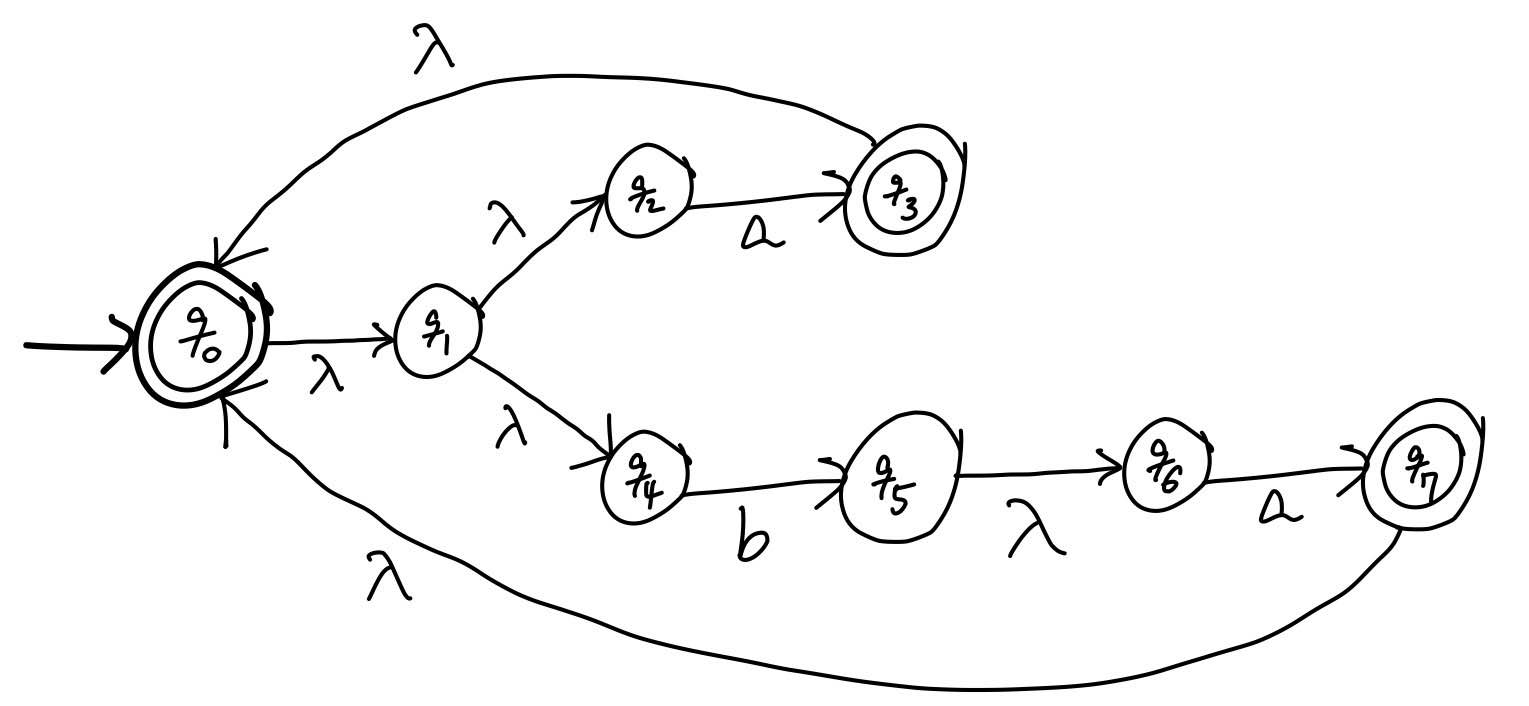
\includegraphics[scale=0.2]{6.2}

            6.6 $(000)^*$

            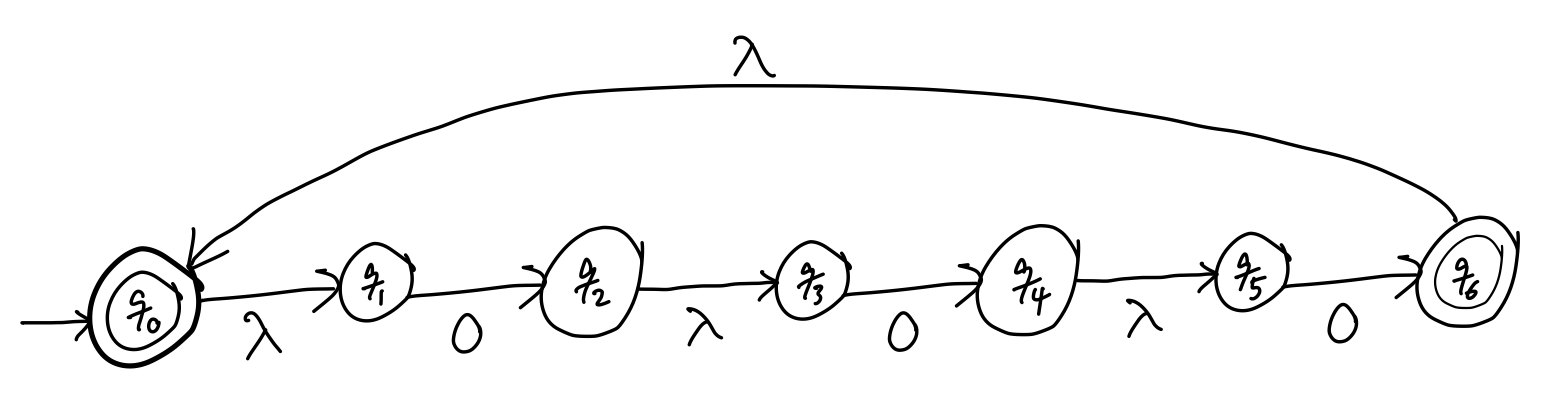
\includegraphics[scale=0.35]{6.6}

            6.9 $(0+1)^* 0(0+1)^2$

            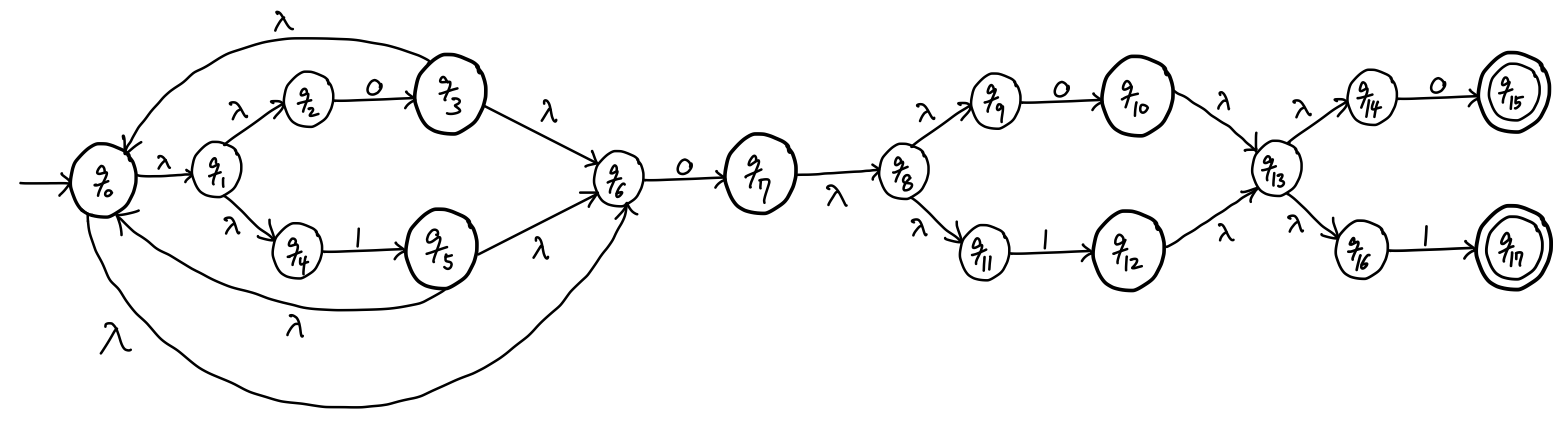
\includegraphics[scale=0.5]{6.9}

      \item Construct DFAs for the following languages and use the state elimination algorithm in this chapter to create a regular expression for each. Show the intermediate steps as you eliminate each state along the way.

            6.13 $\left\{w \in\{0,1\}^*: w\right.$ has at least two 1 s$\}$

            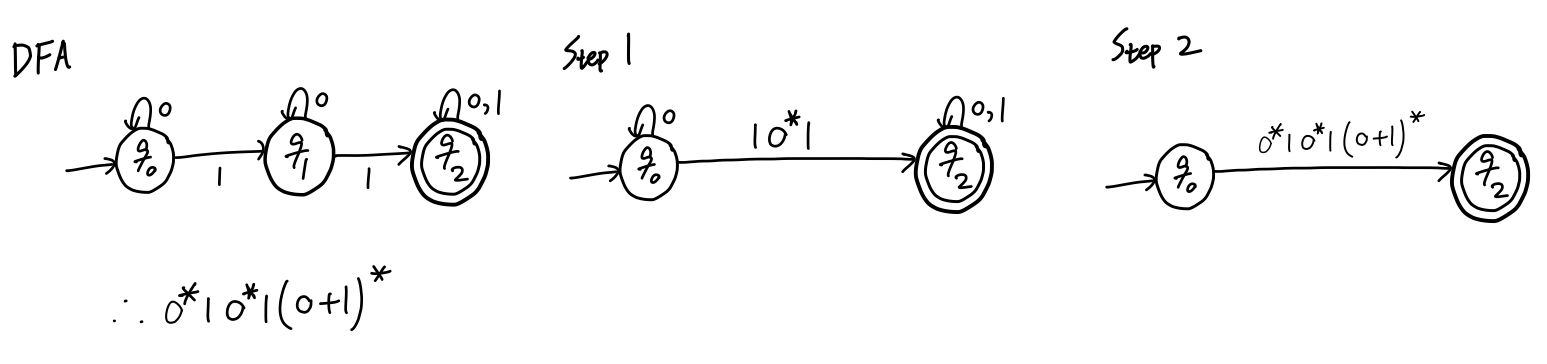
\includegraphics[scale=0.5]{6.13}


            6.15 $\left\{w \in\{0,1\}^*:\right.$ the number of 0 s in $w$ is divisible by 3$\}$

            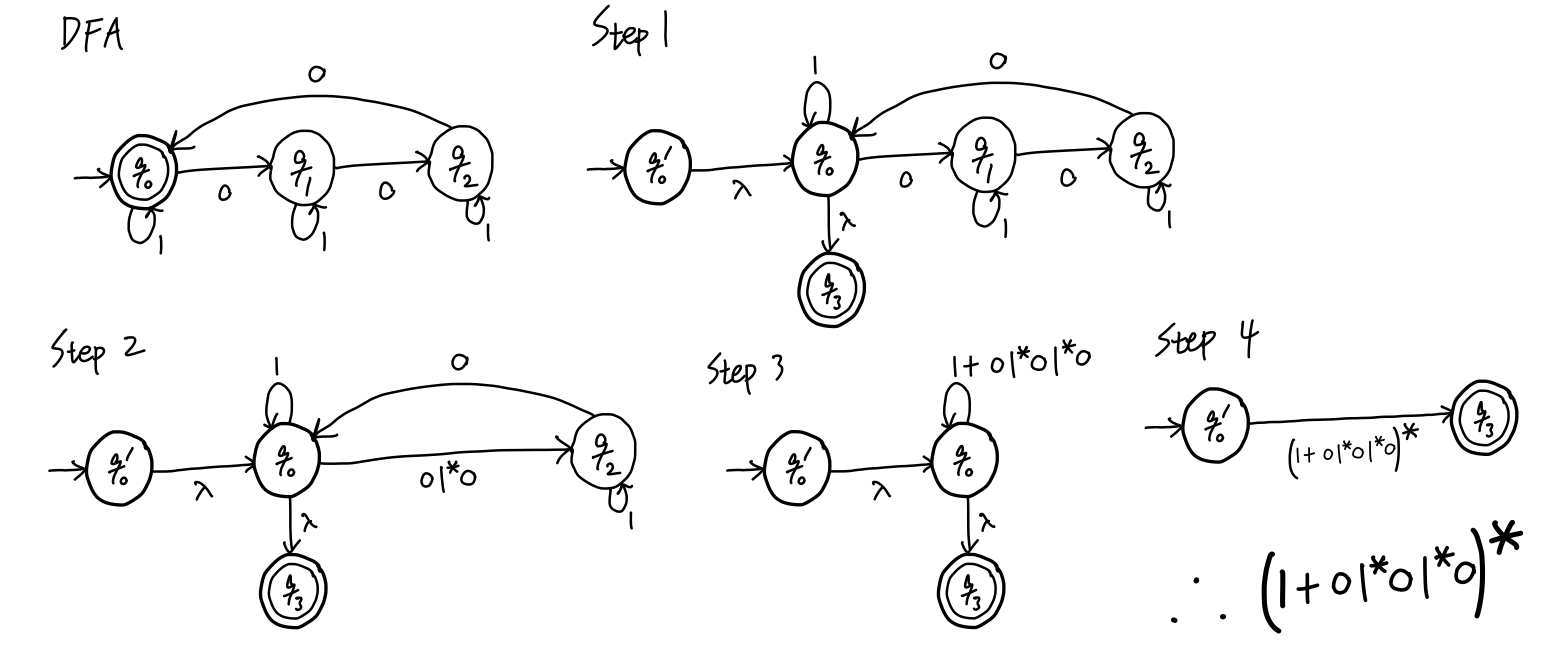
\includegraphics[scale=0.45]{6.15}


            6.16 $\left\{w \in\{0,1\}^*: w\right.$ does not have 01 as a substring $\}$

            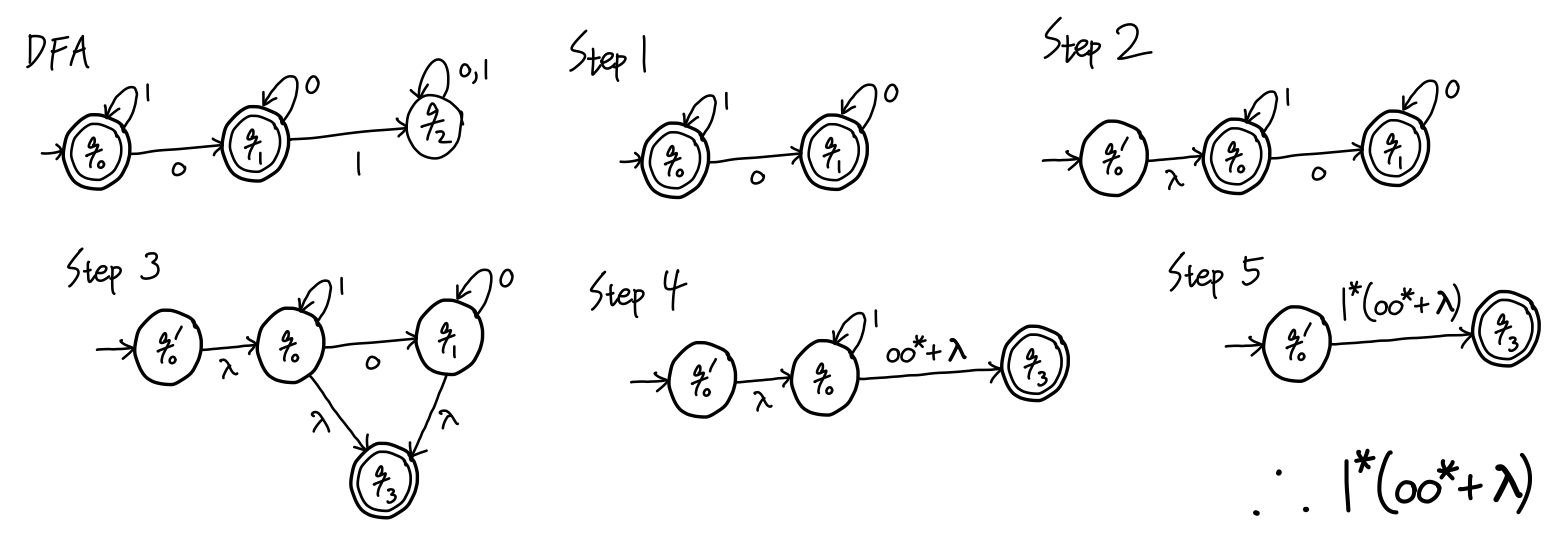
\includegraphics[scale=0.5]{6.16}

            \newpage

            7.2 Show that if $x$ and $y$ are odd length strings and $z$ is an even length string that $x y z$ is an even length string.


            Let $x$ and $y$ be odd length of strings and $z$ be an even length string.\\
            WTS that xyz is an even length of string.\\
            By the def. 7.2 in the text book, we know that there exist some integers p, q $\geq$ 0 such that $|x|=2 p+1,|y|=2 q+1$.\\
            Also, by the def. 7.1 in the text book, we know that there exists some integer r $\geq$ 0 such that $|z|=2 r$.\\
            Then, the length of the string $x y z$ is the sum of the lengths of $x, y$, and $z$, or $2 p+1+2 q+1+2 r=2(p+q+r+1)$. [def. 7.1]\\
            Since we can write the length of $x y z$ as $2s$ (where $s=p+q+r+1 \geq 0$ is an integer), this means that it follows by def 7.1 that $x y z$ is an even length string. $Q.E.D.$\\


            7.8 Show that for all $n \geq 3,4 n^2+6 n \leq 2 n^3$.

            Let us assume that $n \geq 3$. Then we can write
            $$
                  \begin{aligned}
                        4 n^2+6 n & \leq 4 n^2+2 n^2
                                  & {\left[\text { as } 6 n \leq 2 n^2 \text { since } 3 \leq n\right] } \\
                                  & = 6 n^2 \quad[\text { math }]                                        \\
                                  & \leq 2 n^3 \quad[\text { as } 3 \leq n],
                  \end{aligned}
            $$

            which shows that $4 n^2+6 n \leq 2 n^3$.
            Thus, $4 n^2+6 n$ is at most $2 n^3$ for all $n \geq 3$. $Q.E.D.$\\

            7.10 Define the $N O R$ operation as $\operatorname{NOR}\left(L_1, L_2\right)=\left\{x: x \notin L_1 \wedge x \notin L_2\right\}$. Show that regular languages are closed under the $N O R$ operator.

            Suppose $L_1$ and $L_2$ are regular languages.\\
            WTS $\operatorname{NOR}\left(L_1, L_2\right)=\left\{x: x \notin L_1 \wedge x \notin L_2\right\}$ is regular.\\
            By the proof of theorem which was demonstrated in class that regular languages are closed under union, we know that
            $\left\{x: x \in L_1\right\} \cup \left\{x:x \in L_2\right\} = \left\{x: x \in L_1 \vee x \in L_2\right\}$ is regular.\\
            Also by the proof of theorem which was demonstrated in class that regular languages are closed under complement, we know that $\left\{x: x \in L_1 \vee x \in L_2\right\}^c = \left\{x: x \notin L_1 \wedge x \notin L_2\right\}$ is regular. \quad[\text { De Morgan's laws }]\\
            Thus, regular languages are closed under the $N O R$ operator by the theorems above. $Q.E.D.$

\end{enumerate}

\newpage

\section*{2 \quad References}

\begin{enumerate}[label={}]

      \item I have used the following external resource in purpose of learning general mechanism and procedure of state elimination algorithm for 5.20, 5.24, 6.13, 6.15, 6.16
      \item \url{https://courses.cs.washington.edu/courses/cse311/14sp/kleene.pdf}


\end{enumerate}
\end{document}